% Chapter: 需求分析

\chapter{需求分析}
  \label{chap:需求分析}

\section{综述}
  \label{sec:综述}
    我的项目是开发一个商城,分为三大模块,分别由三个底部菜单进入。第一大模块是商城部分,由一个列表展现页、店铺详情页、支付详情页和支付成功页组成,可以实现完整的一套购买流程:进入商城 -> 填写订单 -> 支付 -> 支付成功。第二大模块是艾灸文化部分,主要用来推送软文,传播艾灸保健的文化,扩展人们的知识面,由一个文章列表页和文章详情页组成,文章详情页中可以给文章点赞、收藏等。第三大模块则是我的空间部分,保存了个人的基本信息、收藏与保健记录等。
    \par
    每个页面都有自己的设计图,这是由设计师设计的,我主要负责用代码一行一行去实现各个样式细节,并且还要有交互功能以及各个页面的业务逻辑,下面就来一一介绍各个要页面的功能。

\clearpage
\section{商城模块}
  \label{sec:商城模块}
    \subsection{首页}
      \label{subsec:首页}
        我们先来看下首页的设计图(\ref{fig:home_dsn}),首页是客户打开商城时默认进入的页面,从服务器获取数据信息,以列表的形式展现商城的一些基本信息,包括店铺的缩略图、店名、艾灸服务的价格、其他一些服务及价格、店的地理位置等,而且可以判断根据按钮的颜色判断客户是否在商城预定过,然后点击商城就可以进入店铺内部。
        \begin{figure}[htbp]
          \centering
          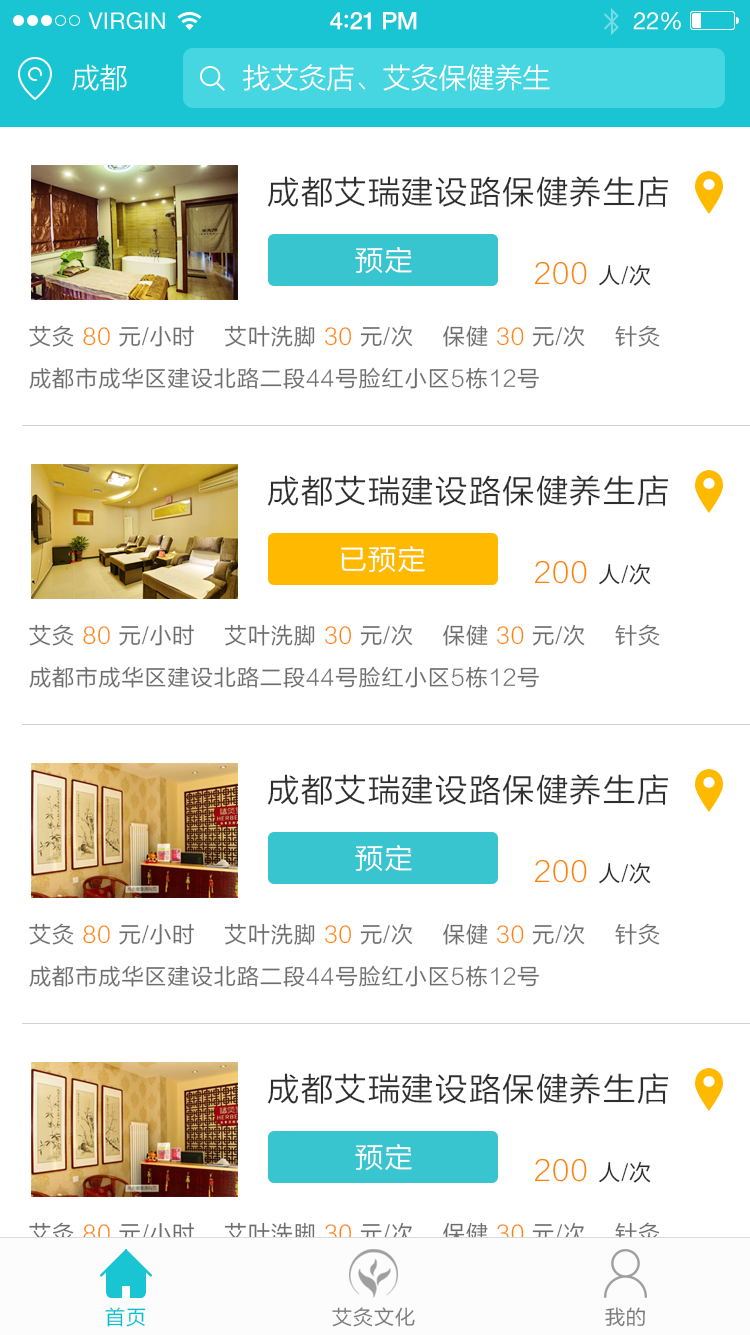
\includegraphics[width=8cm]{./img/home_dsn.jpg}
          \caption{首页的设计图}
          \label{fig:home_dsn}
        \end{figure}

    \subsection{店铺详情页}
      \label{subsec:店铺详情页}
        店铺详情页与下一页的支付页是一个完整的下单与支付流程。店铺详情页展示了一个店铺内部的详细信息,如图(\ref{fig:strdetail_dsn}),包括店铺的内部装饰图、店铺的具体的服务与价格,客户可以在这里勾选服务与预定的日期,以及进行预定操作,预定过程下一页还会继续,用于填写个人的基本信息。
        \begin{figure}[htbp]
          \centering
          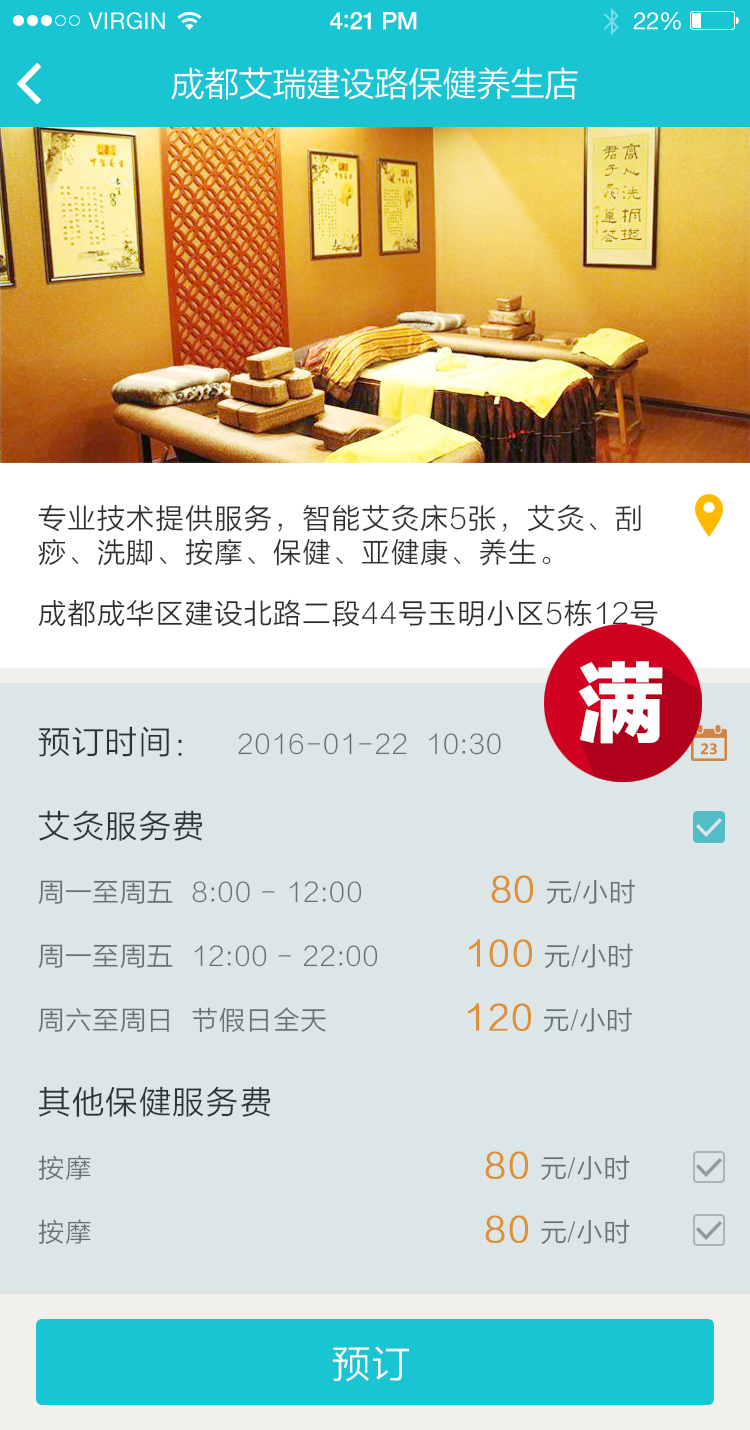
\includegraphics[width=8cm]{./img/strdetail_dsn.png}
          \caption{店铺详情页的设计图}
          \label{fig:strdetail_dsn}
        \end{figure}

    \subsection{支付页}
      \label{subsec:支付页}
        支付页继续上一页的操作,支付页的设计图如图(\ref{fig:pay_dsn}),上一页主要选择了预定的服务,这一页来选择各个服务的人数,选择人数的同时,上面的总价一栏会实时显示总价;接下来是个人信息的填写,包括姓名与电话;最后是选择支付方式,支持微信和支付宝支付,点击最后的支付按钮即可完成支付,并跳转到支付成功的提示页面。
        \begin{figure}[htbp]
          \centering
          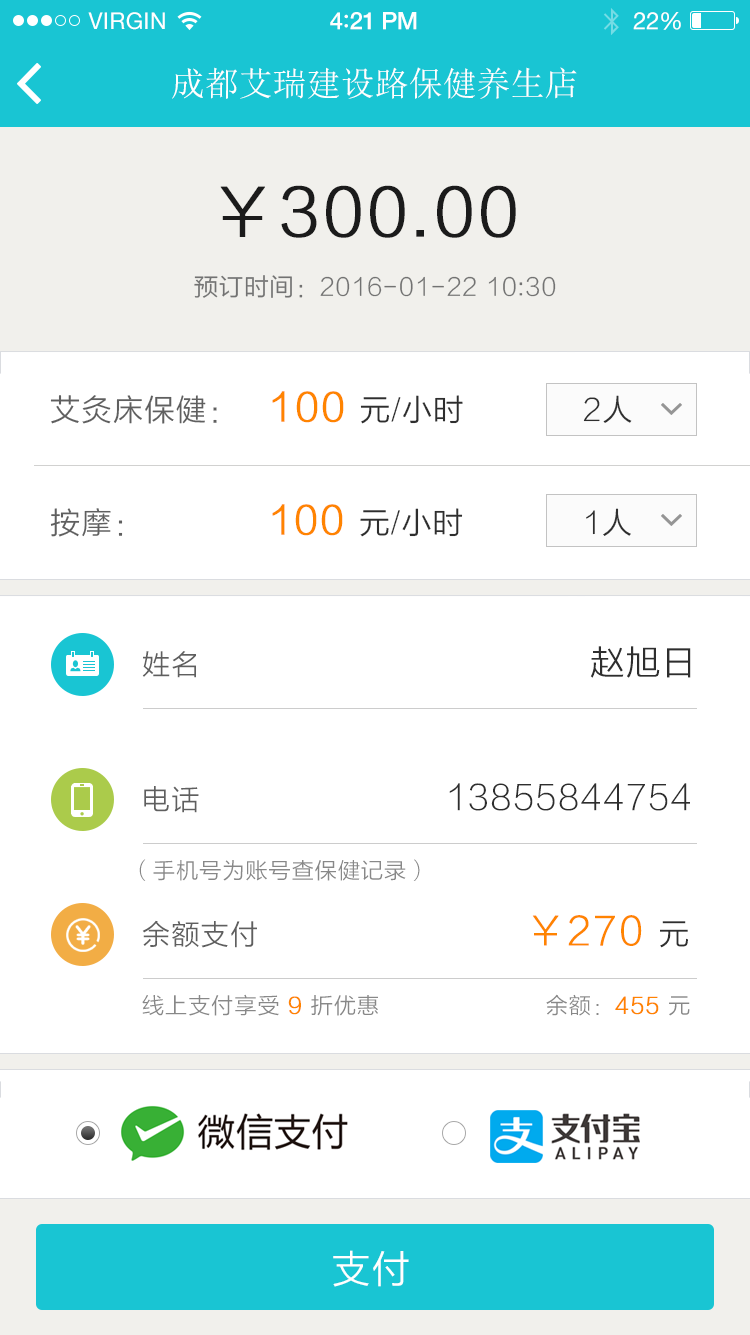
\includegraphics[width=8cm]{./img/pay_dsn.png}
          \caption{支付页设计图}
          \label{fig:pay_dsn}
        \end{figure}

    \subsection{支付成功页}
      \label{subsec:支付成功页}
        支付成功页主要功能除了提示客户已经购买成功,还包括了分享功能,如图(\ref{fig:pay_successful_dsn}),可以分享到微信、微博、QQ 空间,分享成功的同时可以奖励艾灸币,提交到服务器保存,客户可以用来兑换现金。
        \begin{figure}[htbp]
          \centering
          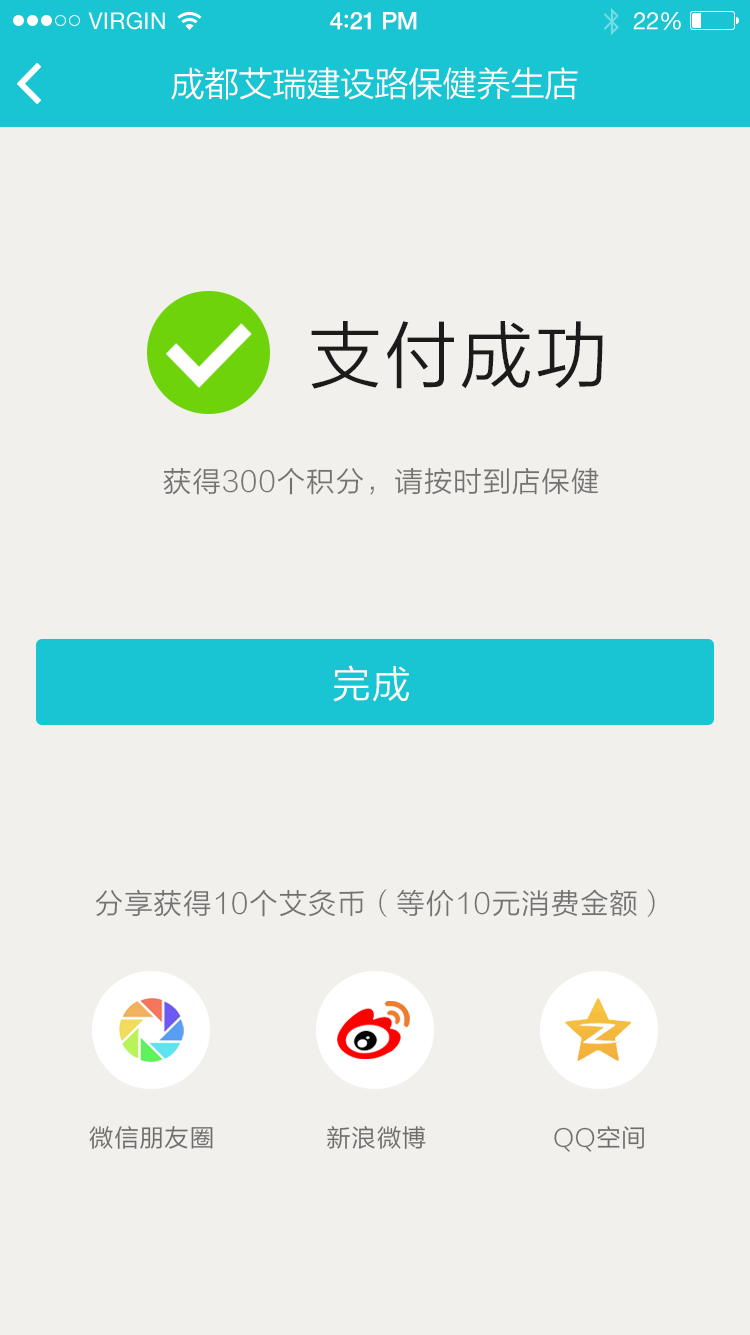
\includegraphics[width=8cm]{./img/pay_successful_dsn.png}
          \caption{支付成功页的设计图}
          \label{fig:pay_successful_dsn}
        \end{figure}

\clearpage
\section{文章模块}
  \label{sec:文章模块}
    \subsection{文章列表页}
      \label{subsec:文章列表页}
        文章列表页的设计图如图(\ref{fig:artlist_dsn}),
        \begin{figure}[htbp]
          \centering
          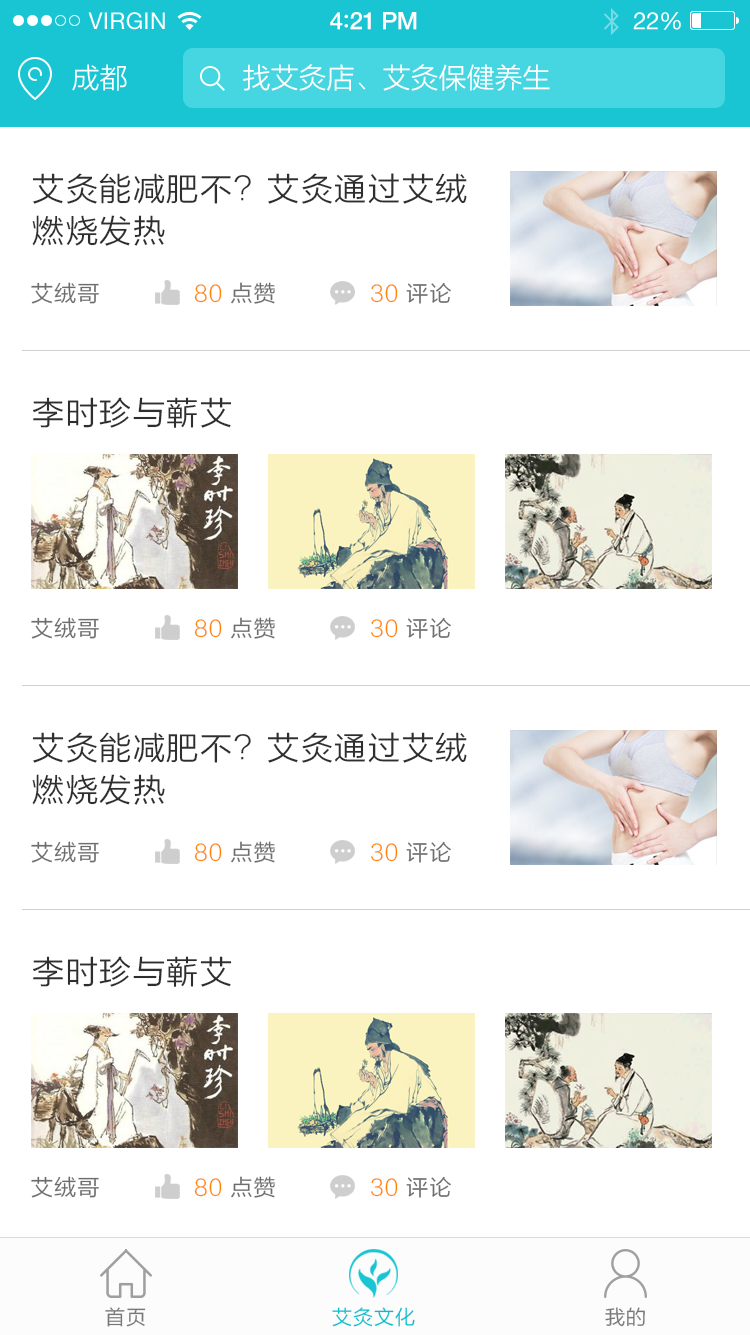
\includegraphics[width=8cm]{./img/artlist_dsn.png}
          \caption{文章列表页的设计图}
          \label{fig:artlist_dsn}
        \end{figure}
        此页面以列表的形式展示了最近的一些文章,每项都显示了文章的一些简要信息,如文章标题、图片、作者、点赞数与评论数等,点击就可进入文章的详情页。


    \subsection{文章详情页}
      \label{subsec:文章详情页}
        文章详情页的设计图如图(\ref{fig:artdetail_dsn}),客户可以在此页浏览文章,喜欢的话可以点击上面的点赞收藏图标进行收藏,收藏的文章会保存在我的空间的收藏一栏的位置。
        \begin{figure}[htbp]
          \centering
          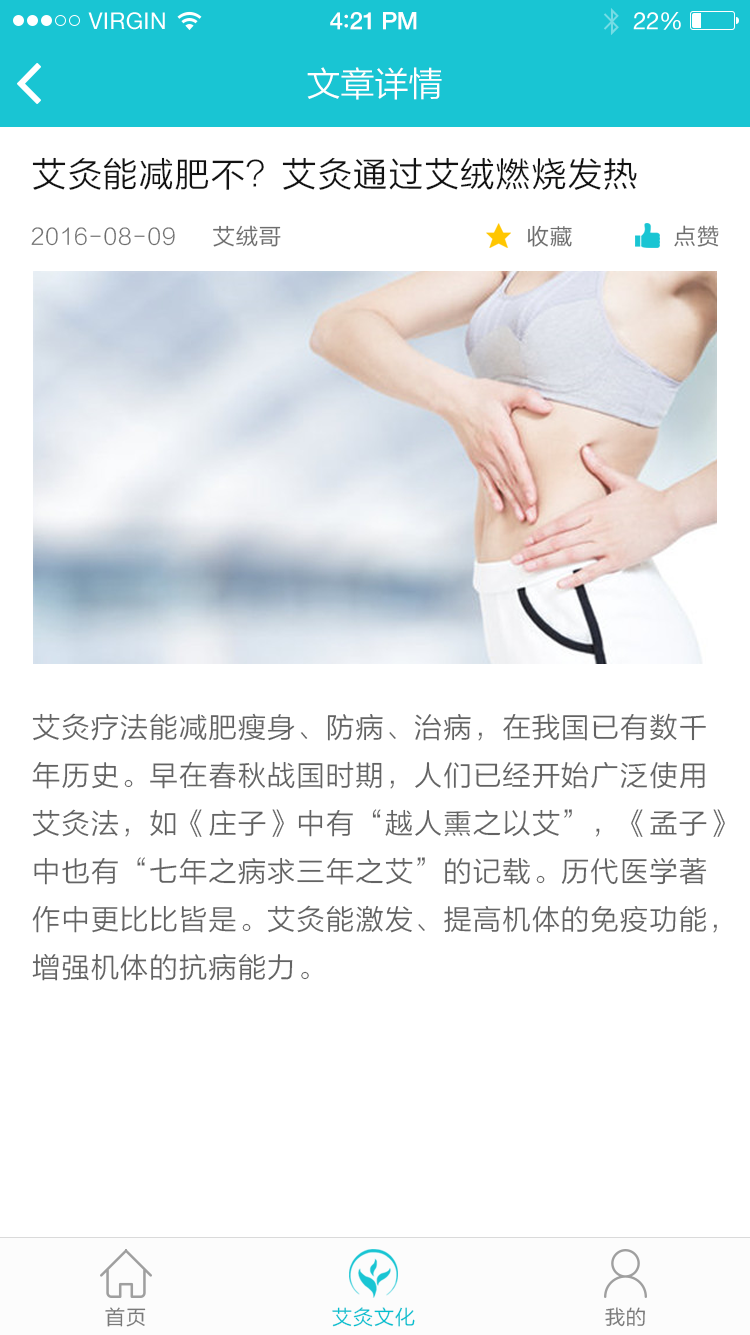
\includegraphics[width=8cm]{./img/artdetail_dsn.png}
          \caption{文章详情页的设计图}
          \label{fig:artdetail_dsn}
        \end{figure}

\clearpage
\section{我的空间模块}
  \label{sec:我的空间模块}
    \subsection{我的空间页}
      \label{subsec:我的空间页}
        我的空间页的设计图如图(\ref{fig:mine_dsn}),此页展示了用户的一些基本信息,如昵称、头像,还通过气泡提示的方法展示了客户保健的次数、收藏的店铺和文章的个数以及积分数。下半部分是一些导航菜单,分别可以进入个人的消费记录页面、我的收藏页面、设置信息的页面。
        \begin{figure}[htbp]
          \centering
          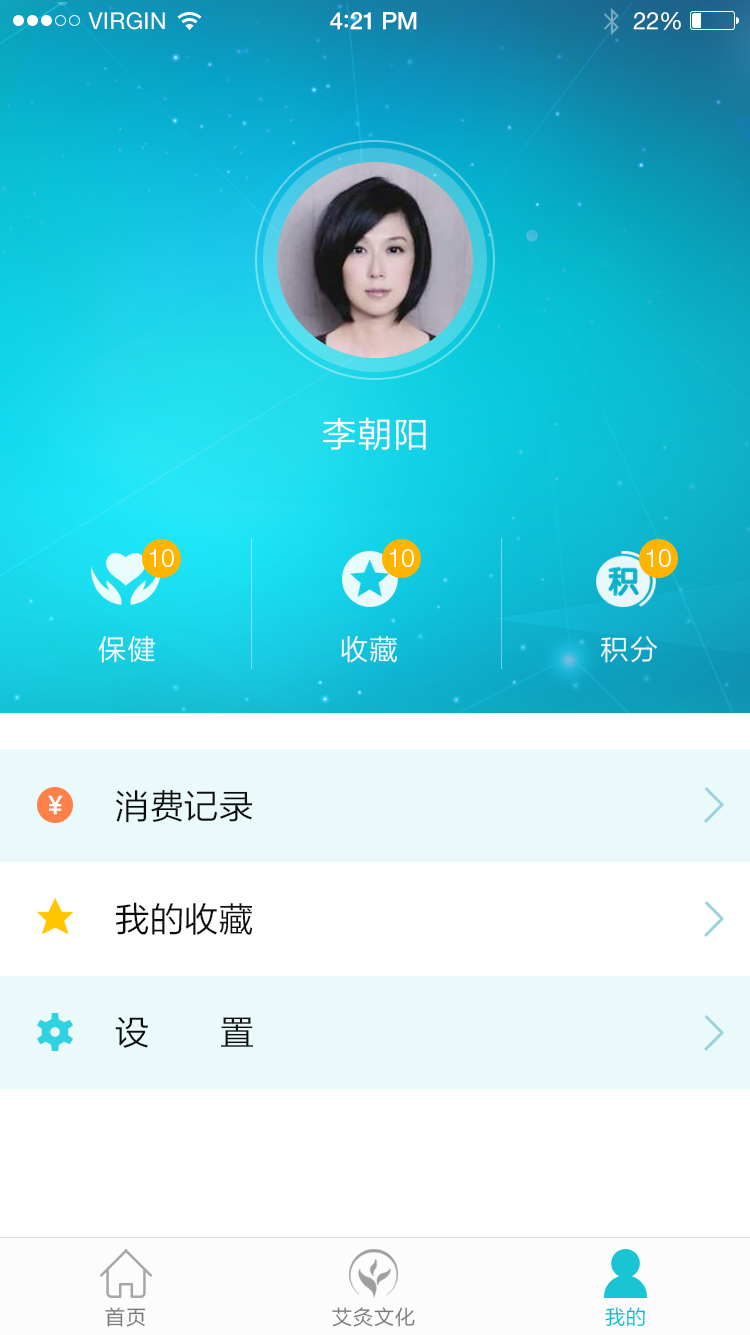
\includegraphics[width=8cm]{./img/mine_dsn.png}
          \caption{我的空间页}
          \label{fig:mine_dsn}
        \end{figure}

    \subsection{消费记录页}
      \label{subsec:消费记录页}
        消费记录记录了个人的消费情况,以流水线的样式展现,展示的信息包括店名、保健的人数、时间、费用以及积分等,积分将来可以用于兑换艾灸币,顶部还展示了总的消费情况,总的积分。设计图如图(\ref{fig:record_dsn})。
        \begin{figure}[htbp]
          \centering
          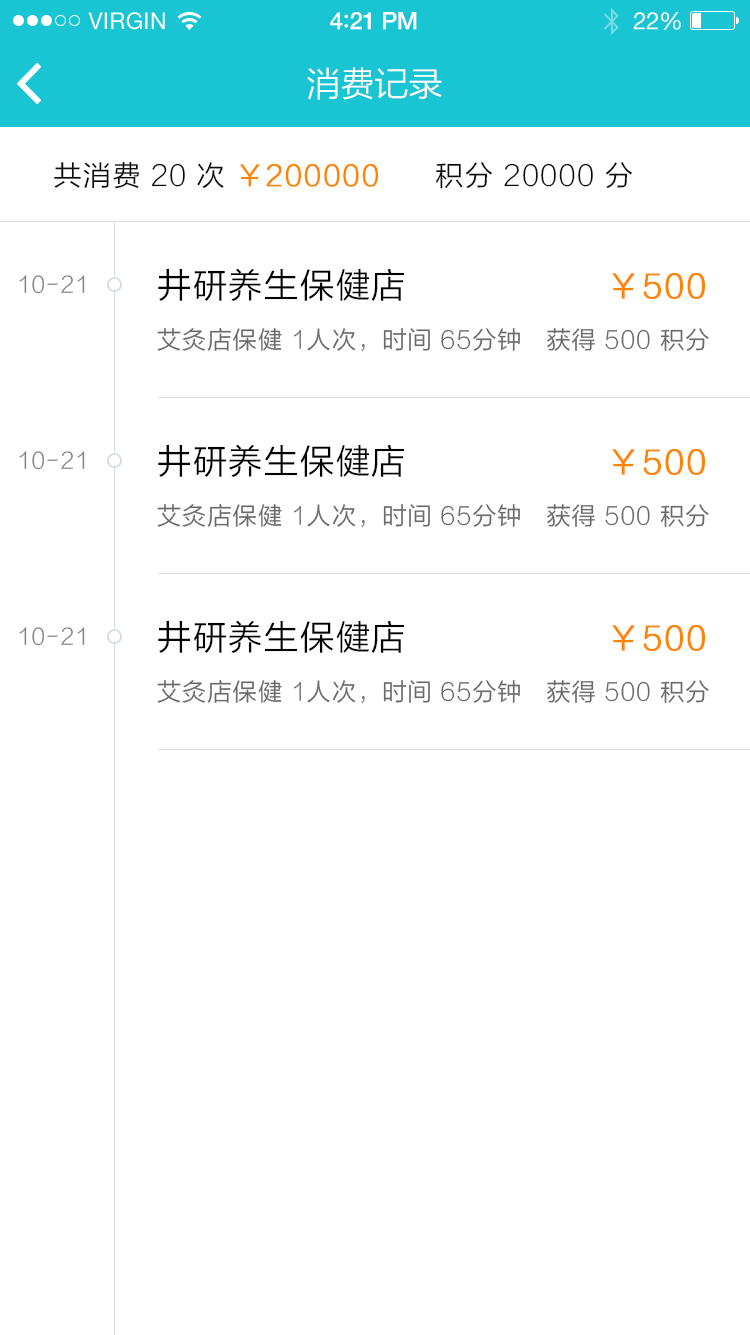
\includegraphics[width=8cm]{./img/record_dsn.png}
          \caption{消费记录页}
          \label{fig:record_dsn}
        \end{figure}

    \subsection{设置页}
      \label{subsec:设置页}
        设置页的设计图如图(\ref{fig:setting_dsn})在这一页中,客户可以设置自己的基本信息,包括昵称、手机号、登录密码等。
        \begin{figure}[htbp]
          \centering
          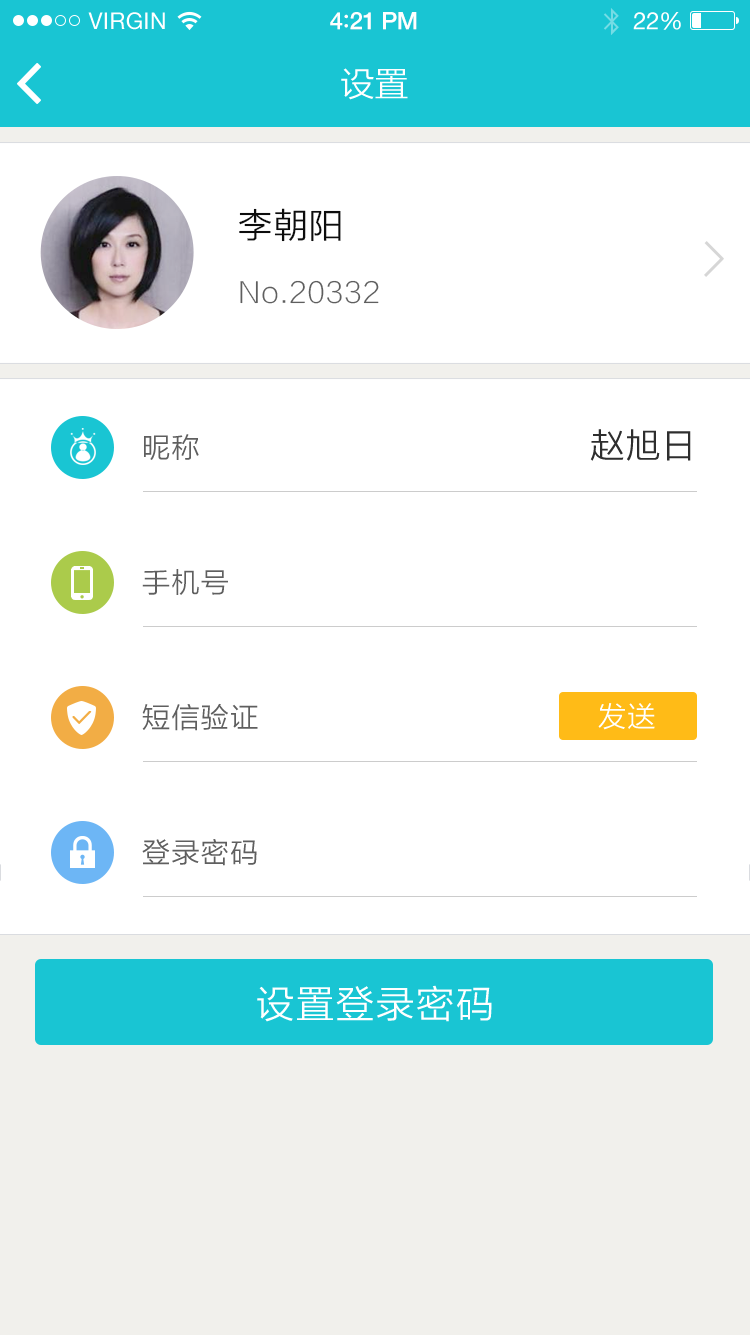
\includegraphics[width=8cm]{./img/setting_dsn.png}
          \caption{设置页的设计图}
          \label{fig:setting_dsn}
        \end{figure}

\clearpage
\section{本章小结}
  \label{sec:需求小结}
    本章结合设计图分析了项目的基本需求,展示了一个网上商城应该具备的基本功能。有了基本需求就可以开发了,不过开发前需要进行充足的准备,包括基本知识技能的学习、工具的选择与使用,下面一章我们就来简要介绍项目开发用到的必要知识与工具。

